\documentclass[border=10pt]{standalone}

\usepackage[utf8]{inputenc}
\usepackage[english]{babel}
\usepackage{tikz}
\usetikzlibrary{positioning, arrows.meta, fit}

\begin{document}
	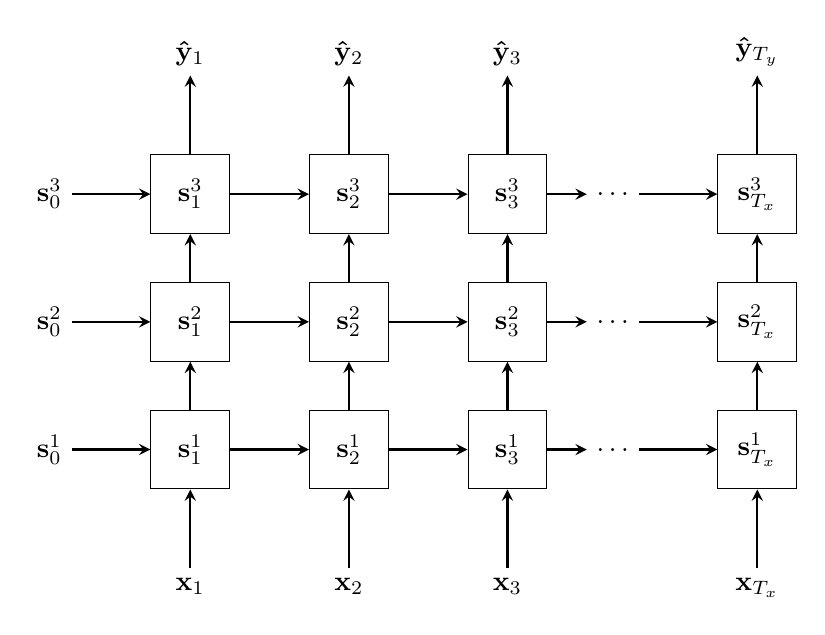
\begin{tikzpicture}
		% layer1 rnn
		\node[rectangle, draw, minimum height=1cm, minimum width=1cm] (al11) {$\mathbf{s}^{1}_{1}$};
		\node[left=of al11] (al10) {$\mathbf{s}^{1}_{0}$};
		\node[rectangle, right=of al11, draw, minimum height=1cm, minimum width=1cm] (al12) {$\mathbf{s}^{1}_{2}$};
		\node[rectangle, right=of al12, draw, minimum height=1cm, minimum width=1cm] (al13) {$\mathbf{s}^{1}_{3}$};
		\node[rectangle, right=0.5 of al13] (al14) {$\dots$};
		\node[rectangle, right= of al14, draw, minimum height=1cm, minimum width=1cm] (al1tx) {$\mathbf{s}^{1}_{T_{x}}$};
		% layer2 rnn
		\node[above=of al10] (al20) {$\mathbf{s}^{2}_{0}$};
		\node[rectangle, right=of al20, draw, minimum height=1cm, minimum width=1cm] (al21) {$\mathbf{s}^{2}_{1}$};
		\node[rectangle, right=of al21, draw, minimum height=1cm, minimum width=1cm] (al22) {$\mathbf{s}^{2}_{2}$};
		\node[rectangle, right=of al22, draw, minimum height=1cm, minimum width=1cm] (al23) {$\mathbf{s}^{2}_{3}$};
		\node[rectangle, right=0.5 of al23] (al24) {$\dots$};
		\node[rectangle, right= of al24, draw, minimum height=1cm, minimum width=1cm] (al2tx) {$\mathbf{s}^{2}_{T_{x}}$};
		% layer3 rnn
		\node[above=of al20] (al30) {$\mathbf{s}^{3}_{0}$};
		\node[rectangle, right=of al30, draw, minimum height=1cm, minimum width=1cm] (al31) {$\mathbf{s}^{3}_{1}$};
		\node[rectangle, right=of al31, draw, minimum height=1cm, minimum width=1cm] (al32) {$\mathbf{s}^{3}_{2}$};
		\node[rectangle, right=of al32, draw, minimum height=1cm, minimum width=1cm] (al33) {$\mathbf{s}^{3}_{3}$};
		\node[rectangle, right=0.5 of al33] (al34) {$\dots$};
		\node[rectangle, right= of al34, draw, minimum height=1cm, minimum width=1cm] (al3tx) {$\mathbf{s}^{3}_{T_{x}}$};
		% inputs	
		\node[below=of al11] (X1) {$\mathbf{x}_{1}$};
		\node[below=of al12] (X2) {$\mathbf{x}_{2}$};
		\node[below=of al13] (X3) {$\mathbf{x}_{3}$};
		\node[below=of al1tx] (Xt) {$\mathbf{x}_{T_{x}}$};
		% outputs	
		\node[above=of al31] (y1) {$\mathbf{\hat{y}}_{1}$};
		\node[above=of al32] (y2) {$\mathbf{\hat{y}}_{2}$};
		\node[above=of al33] (y3) {$\mathbf{\hat{y}}_{3}$};
		\node[above=of al3tx] (yt) {$\mathbf{\hat{y}}_{T_{y}}$};
		% forward input arrows	- layer1
		\draw[-stealth, thick] (X1) -- (al11);
		\draw[-stealth, thick] (X2) -- (al12);
		\draw[-stealth, thick] (X3) -- (al13);
		\draw[-stealth, thick] (Xt) -- (al1tx);
		% forward input arrows	- layer2
		\draw[-stealth, thick] (al11) -- (al21);
		\draw[-stealth, thick] (al12) -- (al22);
		\draw[-stealth, thick] (al13) -- (al23);
		\draw[-stealth, thick] (al1tx) -- (al2tx);
		% forward input arrows	- layer3
		\draw[-stealth, thick] (al21) -- (al31);
		\draw[-stealth, thick] (al22) -- (al32);
		\draw[-stealth, thick] (al23) -- (al33);
		\draw[-stealth, thick] (al2tx) -- (al3tx);
		% output rnn
		\draw[-stealth, thick] (al31) -- (y1);
		\draw[-stealth, thick] (al32) -- (y2);
		\draw[-stealth, thick] (al33) -- (y3);
		\draw[-stealth, thick] (al3tx) -- (yt);
		% forward hidden states - layer1
		\draw[-stealth, thick] (al10) -- node[above, pos=0.35] {} (al11);
		\draw[-stealth, thick] (al11) -- node[above, pos=0.35] {} (al12);
		\draw[-stealth, thick] (al12) -- node[above, pos=0.35] {} (al13);
		\draw[-stealth, thick] (al13) -- node[above, pos=0.35] {} (al14);
		\draw[-stealth, thick] (al14) -- node[above, pos=0.35] {} (al1tx);
		% forward hidden states - layer2
		\draw[-stealth, thick] (al20) -- node[above, pos=0.35] {} (al21);
		\draw[-stealth, thick] (al21) -- node[above, pos=0.35] {} (al22);
		\draw[-stealth, thick] (al22) -- node[above, pos=0.35] {} (al23);
		\draw[-stealth, thick] (al23) -- node[above, pos=0.35] {} (al24);
		\draw[-stealth, thick] (al24) -- node[above, pos=0.35] {} (al2tx);
		% forward hidden states - layer2
		\draw[-stealth, thick] (al30) -- node[above, pos=0.35] {} (al31);
		\draw[-stealth, thick] (al31) -- node[above, pos=0.35] {} (al32);
		\draw[-stealth, thick] (al32) -- node[above, pos=0.35] {} (al33);
		\draw[-stealth, thick] (al33) -- node[above, pos=0.35] {} (al34);
		\draw[-stealth, thick] (al34) -- node[above, pos=0.35] {} (al3tx);
	\end{tikzpicture}
\end{document}